\documentclass{article}

\newcommand{\forget}[1]{}


\usepackage[margin=4.00055cm,nohead,a4paper,truedimen,dvips]{geometry}
\usepackage[dvips]{graphicx}
\usepackage{pict2e}
\usepackage{epic}
\usepackage{lscape}
\usepackage{eepic}
\usepackage{tikz}
\usetikzlibrary{shapes,arrows,snakes,calc}

\raggedbottom \setlength{\topskip}{1\topskip plus 5pt} \widowpenalty=8000 \clubpenalty=8000

\addtolength{\textheight}{-3.65\baselineskip}

\begin{document}

\pagenumbering{gobble}

\author{}
\date{}
\title{}


% first column

\newsavebox{\fia}
\savebox{\fia}{


\scalebox{3}{

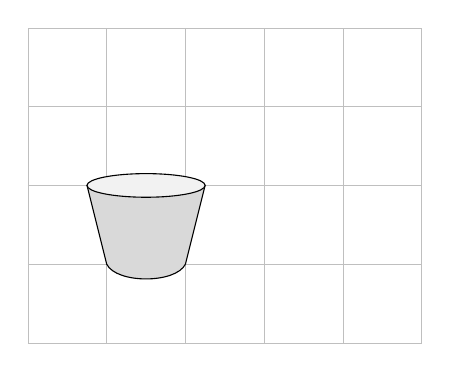
\begin{tikzpicture}

\draw [help lines,lightgray] (0,0) grid (5,4) ;
\draw[fill=gray!30] (1,1) .. controls (1.125,.75) and (1.875,.75) .. (2,1) -- (2.25,2) --  (.75,2) -- (1,1);
\draw[fill=gray!10] (1.5,2) ellipse (.75cm and .15cm) ;

\end{tikzpicture}
}

}

\newsavebox{\fib}
\savebox{\fib}{


\scalebox{3}{

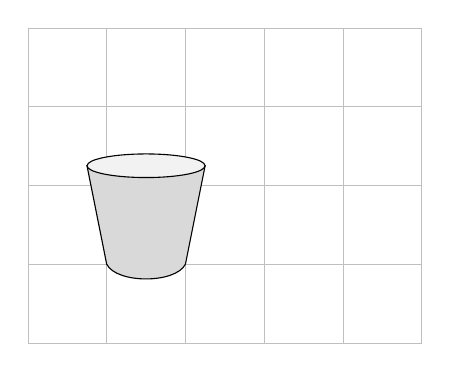
\begin{tikzpicture}

\draw [help lines,lightgray] (0,0) grid (5,4) ;
\draw[fill=gray!30] (1,1) .. controls (1.125,.75) and (1.875,.75) .. (2,1) -- (2.25,2.25) --  (.75,2.25) -- (1,1);
\draw[fill=gray!10] (1.5,2.25) ellipse (.75cm and .15cm) ;

\end{tikzpicture}
}

}

\newsavebox{\fic}
\savebox{\fic}{


\scalebox{3}{

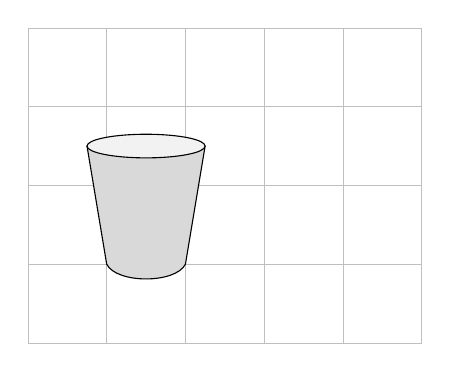
\begin{tikzpicture}

\draw [help lines,lightgray] (0,0) grid (5,4) ;
\draw[fill=gray!30] (1,1) .. controls (1.125,.75) and (1.875,.75) .. (2,1) -- (2.25,2.5) --  (.75,2.5) -- (1,1);
\draw[fill=gray!10] (1.5,2.5) ellipse (.75cm and .15cm) ;

\end{tikzpicture}
}

}

\newsavebox{\fid}
\savebox{\fid}{


\scalebox{3}{

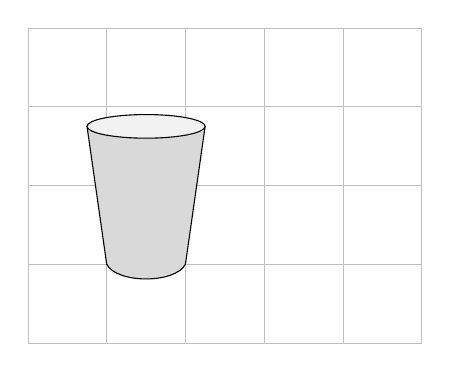
\begin{tikzpicture}

\draw [help lines,lightgray] (0,0) grid (5,4) ;
\draw[fill=gray!30] (1,1) .. controls (1.125,.75) and (1.875,.75) .. (2,1) -- (2.25,2.75) --  (.75,2.75) -- (1,1);
\draw[fill=gray!10] (1.5,2.75) ellipse (.75cm and .15cm) ;

\end{tikzpicture}
}

}

\newsavebox{\fie}
\savebox{\fie}{


\scalebox{3}{

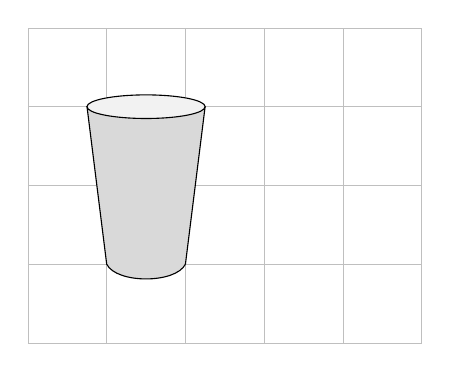
\begin{tikzpicture}

\draw [help lines,lightgray] (0,0) grid (5,4) ;
\draw[fill=gray!30] (1,1) .. controls (1.125,.75) and (1.875,.75) .. (2,1) -- (2.25,3) --  (.75,3) -- (1,1);
\draw[fill=gray!10] (1.5,3) ellipse (.75cm and .15cm) ;

\end{tikzpicture}
}

}

\newsavebox{\fif}
\savebox{\fif}{


\scalebox{3}{

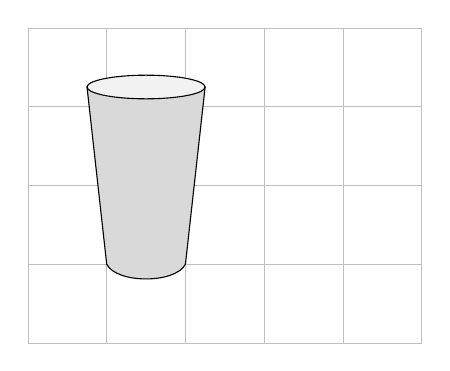
\begin{tikzpicture}

\draw [help lines,lightgray] (0,0) grid (5,4) ;
\draw[fill=gray!30] (1,1) .. controls (1.125,.75) and (1.875,.75) .. (2,1) -- (2.25,3.25) --  (.75,3.25) -- (1,1);
\draw[fill=gray!10] (1.5,3.25) ellipse (.75cm and .15cm) ;

\end{tikzpicture}
}

}

\newsavebox{\fig}
\savebox{\fig}{


\scalebox{3}{

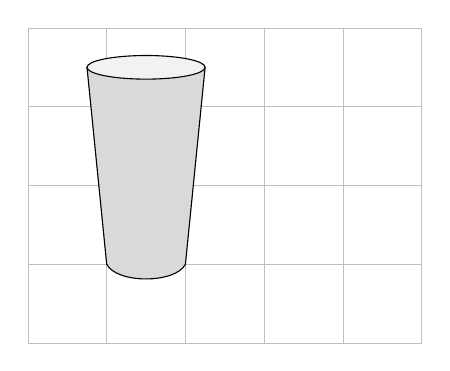
\begin{tikzpicture}

\draw [help lines,lightgray] (0,0) grid (5,4) ;
\draw[fill=gray!30] (1,1) .. controls (1.125,.75) and (1.875,.75) .. (2,1) -- (2.25,3.5) --  (.75,3.5) -- (1,1);
\draw[fill=gray!10] (1.5,3.5) ellipse (.75cm and .15cm) ;

\end{tikzpicture}
}

}


% second column

\newsavebox{\sa}
\savebox{\sa}{


\scalebox{3}{

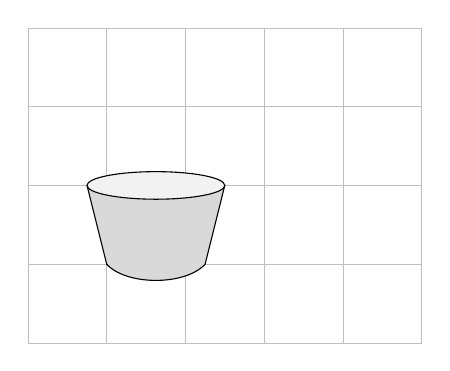
\begin{tikzpicture}

\draw [help lines,lightgray] (0,0) grid (5,4) ;
\draw[fill=gray!30] (1,1) .. controls (1.25,.725) and (2,.725) .. (2.25,1) -- (2.5,2) --  (.75,2) -- (1,1);
\draw[fill=gray!10] (1.625,2) ellipse (.875cm and .175cm) ;

\end{tikzpicture}
}

}


\newsavebox{\seb}
\savebox{\seb}{


\scalebox{3}{

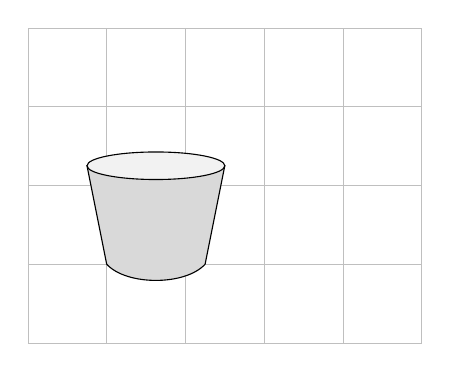
\begin{tikzpicture}

\draw [help lines,lightgray] (0,0) grid (5,4) ;
\draw[fill=gray!30] (1,1) .. controls (1.25,.725) and (2,.725) .. (2.25,1) -- (2.5,2.25) --  (.75,2.25) -- (1,1);
\draw[fill=gray!10] (1.625,2.25) ellipse (.875cm and .175cm) ;

\end{tikzpicture}
}

}

\newsavebox{\secc}
\savebox{\secc}{


\scalebox{3}{

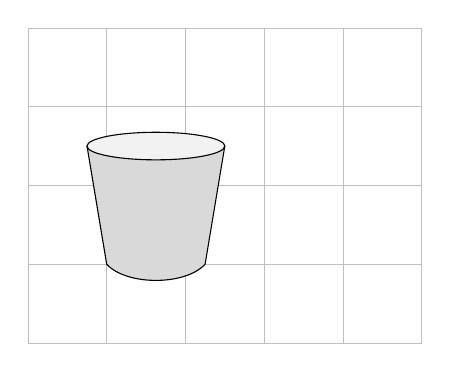
\begin{tikzpicture}

\draw [help lines,lightgray] (0,0) grid (5,4) ;
\draw[fill=gray!30] (1,1) .. controls (1.25,.725) and (2,.725) .. (2.25,1) -- (2.5,2.5) --  (.75,2.5) -- (1,1);
\draw[fill=gray!10] (1.625,2.5) ellipse (.875cm and .175cm) ;

\end{tikzpicture}
}

}

\newsavebox{\secd}
\savebox{\secd}{


\scalebox{3}{

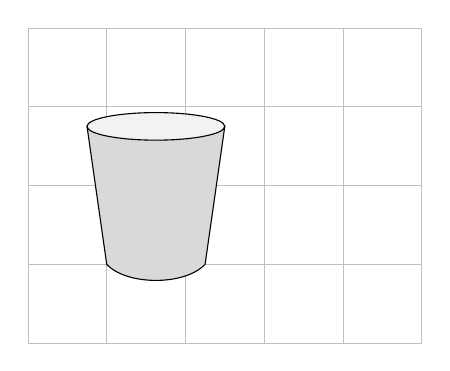
\begin{tikzpicture}

\draw [help lines,lightgray] (0,0) grid (5,4) ;
\draw[fill=gray!30] (1,1) .. controls (1.25,.725) and (2,.725) .. (2.25,1) -- (2.5,2.75) --  (.75,2.75) -- (1,1);
\draw[fill=gray!10] (1.625,2.75) ellipse (.875cm and .175cm) ;

\end{tikzpicture}
}

}

\newsavebox{\see}
\savebox{\see}{


\scalebox{3}{

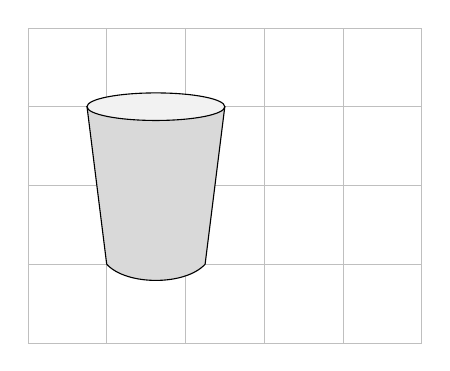
\begin{tikzpicture}

\draw [help lines,lightgray] (0,0) grid (5,4) ;
\draw[fill=gray!30] (1,1) .. controls (1.25,.725) and (2,.725) .. (2.25,1) -- (2.5,3) --  (.75,3) -- (1,1);
\draw[fill=gray!10] (1.625,3) ellipse (.875cm and .175cm) ;

\end{tikzpicture}
}

}

\newsavebox{\sef}
\savebox{\sef}{


\scalebox{3}{

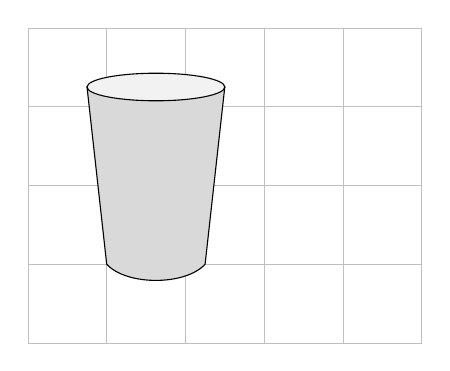
\begin{tikzpicture}

\draw [help lines,lightgray] (0,0) grid (5,4) ;
\draw[fill=gray!30] (1,1) .. controls (1.25,.725) and (2,.725) .. (2.25,1) -- (2.5,3.25) --  (.75,3.25) -- (1,1);
\draw[fill=gray!10] (1.625,3.25) ellipse (.875cm and .175cm) ;

\end{tikzpicture}
}

}

\newsavebox{\sg}
\savebox{\sg}{


\scalebox{3}{

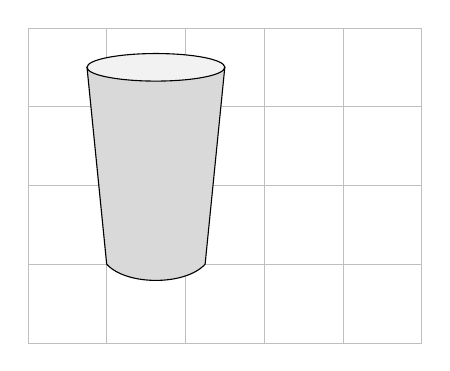
\begin{tikzpicture}

\draw [help lines,lightgray] (0,0) grid (5,4) ;
\draw[fill=gray!30] (1,1) .. controls (1.25,.725) and (2,.725) .. (2.25,1) -- (2.5,3.5) --  (.75,3.5) -- (1,1);
\draw[fill=gray!10] (1.625,3.5) ellipse (.875cm and .175cm) ;

\end{tikzpicture}
}

}


% third column

\newsavebox{\tira}
\savebox{\tira}{


\scalebox{3}{

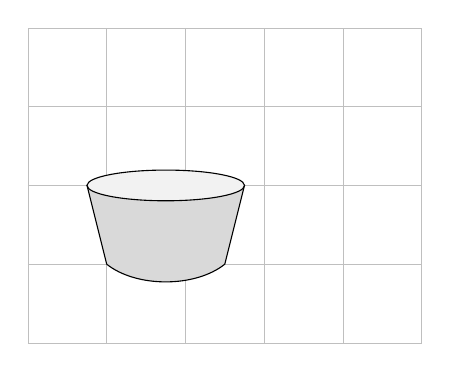
\begin{tikzpicture}

\draw [help lines,lightgray] (0,0) grid (5,4) ;
\draw[fill=gray!30] (1,1) .. controls (1.375,.7) and (2.125,.7) .. (2.5,1) -- (2.75,2) --  (.75,2) -- (1,1);
\draw[fill=gray!10] (1.75,2) ellipse (1cm and .195cm) ;

\end{tikzpicture}
}

}

\newsavebox{\tirb}
\savebox{\tirb}{


\scalebox{3}{

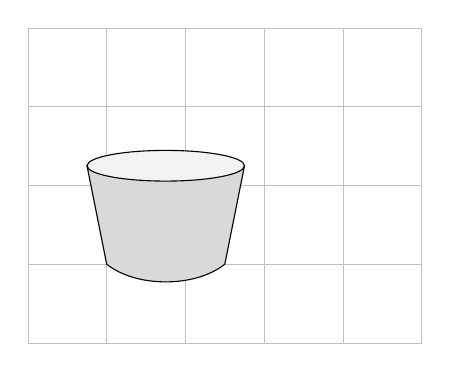
\begin{tikzpicture}

\draw [help lines,lightgray] (0,0) grid (5,4) ;
\draw[fill=gray!30] (1,1) .. controls (1.375,.7) and (2.125,.7)  .. (2.5,1) -- (2.75,2.25) --  (.75,2.25) -- (1,1);
\draw[fill=gray!10] (1.75,2.25) ellipse (1cm and .195cm) ;

\end{tikzpicture}
}

}

\newsavebox{\tirc}
\savebox{\tirc}{


\scalebox{3}{

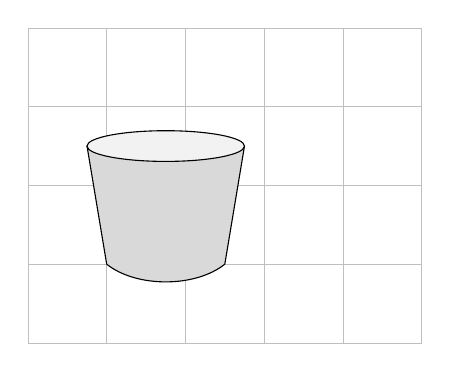
\begin{tikzpicture}

\draw [help lines,lightgray] (0,0) grid (5,4) ;
\draw[fill=gray!30] (1,1) .. controls (1.375,.7) and (2.125,.7)  .. (2.5,1) -- (2.75,2.5) --  (.75,2.5) -- (1,1);
\draw[fill=gray!10] (1.75,2.5) ellipse (1cm and .195cm) ;

\end{tikzpicture}
}

}

\newsavebox{\tird}
\savebox{\tird}{


\scalebox{3}{

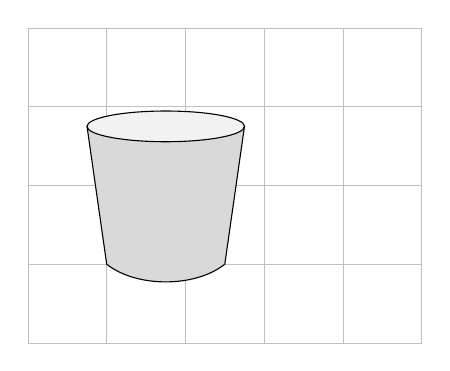
\begin{tikzpicture}

\draw [help lines,lightgray] (0,0) grid (5,4) ;
\draw[fill=gray!30] (1,1) .. controls (1.375,.7) and (2.125,.7)  .. (2.5,1) -- (2.75,2.75) --  (.75,2.75) -- (1,1);
\draw[fill=gray!10] (1.75,2.75) ellipse (1cm and .195cm) ;

\end{tikzpicture}
}

}

\newsavebox{\tire}
\savebox{\tire}{


\scalebox{3}{

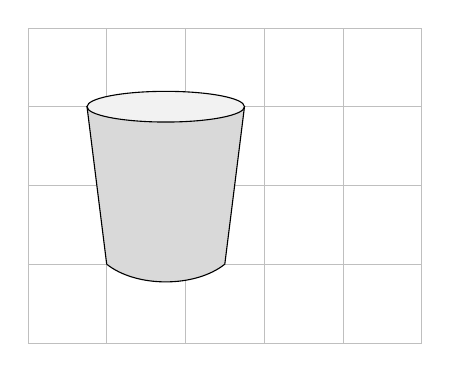
\begin{tikzpicture}

\draw [help lines,lightgray] (0,0) grid (5,4) ;
\draw[fill=gray!30] (1,1) .. controls (1.375,.7) and (2.125,.7) .. (2.5,1) -- (2.75,3) --  (.75,3) -- (1,1);
\draw[fill=gray!10] (1.75,3) ellipse (1cm and .195cm) ;

\end{tikzpicture}
}

}

\newsavebox{\tirf}
\savebox{\tirf}{


\scalebox{3}{

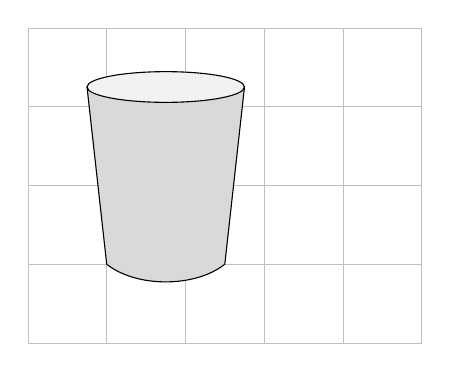
\begin{tikzpicture}

\draw [help lines,lightgray] (0,0) grid (5,4) ;
\draw[fill=gray!30] (1,1) .. controls (1.375,.7) and (2.125,.7)  .. (2.5,1) -- (2.75,3.25) --  (.75,3.25) -- (1,1);
\draw[fill=gray!10] (1.75,3.25) ellipse (1cm and .195cm) ;

\end{tikzpicture}
}

}

\newsavebox{\tirg}
\savebox{\tirg}{


\scalebox{3}{

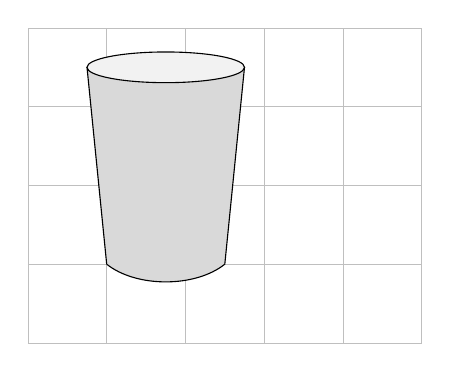
\begin{tikzpicture}

\draw [help lines,lightgray] (0,0) grid (5,4) ;
\draw[fill=gray!30] (1,1) .. controls (1.375,.7) and (2.125,.7) .. (2.5,1) -- (2.75,3.5) --  (.75,3.5) -- (1,1);
\draw[fill=gray!10] (1.75,3.5) ellipse (1cm and .195cm) ;

\end{tikzpicture}
}

}


% fourth column

\newsavebox{\foa}
\savebox{\foa}{


\scalebox{3}{

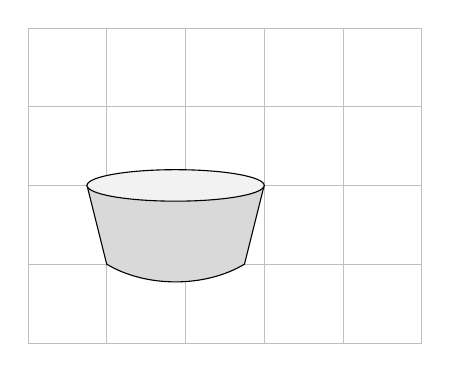
\begin{tikzpicture}

\draw [help lines,lightgray] (0,0) grid (5,4) ;
\draw[fill=gray!30] (1,1) .. controls (1.5,.7) and (2.25,.7) .. (2.75,1) -- (3,2) --  (.75,2) -- (1,1);
\draw[fill=gray!10] (1.875,2) ellipse (1.125cm and .2cm) ;

\end{tikzpicture}
}

}


\newsavebox{\fob}
\savebox{\fob}{


\scalebox{3}{

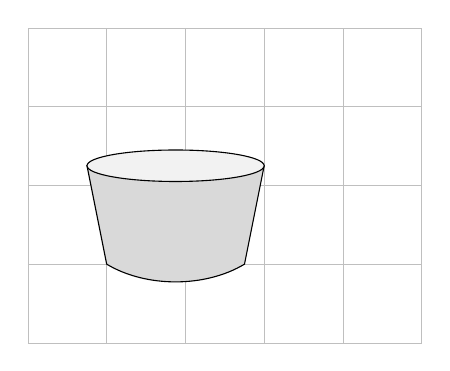
\begin{tikzpicture}

\draw [help lines,lightgray] (0,0) grid (5,4) ;
\draw[fill=gray!30] (1,1) .. controls (1.5,.7) and (2.25,.7) .. (2.75,1) -- (3,2.25) --  (.75,2.25) -- (1,1);
\draw[fill=gray!10] (1.875,2.25) ellipse (1.125cm and .2cm) ;

\end{tikzpicture}
}

}

\newsavebox{\foc}
\savebox{\foc}{


\scalebox{3}{

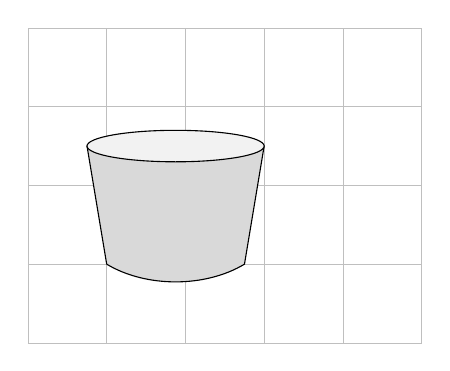
\begin{tikzpicture}

\draw [help lines,lightgray] (0,0) grid (5,4) ;
\draw[fill=gray!30] (1,1) .. controls (1.5,.7) and (2.25,.7) .. (2.75,1) -- (3,2.5) --  (.75,2.5) -- (1,1);
\draw[fill=gray!10] (1.875,2.5) ellipse (1.125cm and .2cm) ;

\end{tikzpicture}
}

}

\newsavebox{\fod}
\savebox{\fod}{


\scalebox{3}{

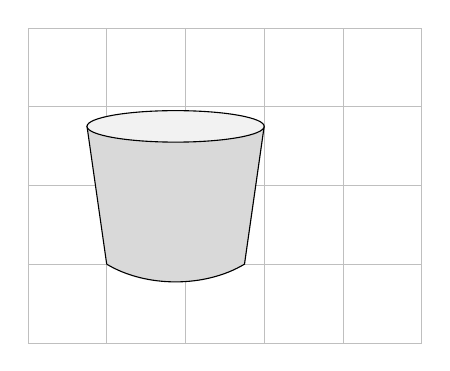
\begin{tikzpicture}

\draw [help lines,lightgray] (0,0) grid (5,4) ;
\draw[fill=gray!30] (1,1) .. controls (1.5,.7) and (2.25,.7) .. (2.75,1) -- (3,2.75) --  (.75,2.75) -- (1,1);
\draw[fill=gray!10] (1.875,2.75) ellipse (1.125cm and .2cm) ;

\end{tikzpicture}
}

}

\newsavebox{\foe}
\savebox{\foe}{


\scalebox{3}{

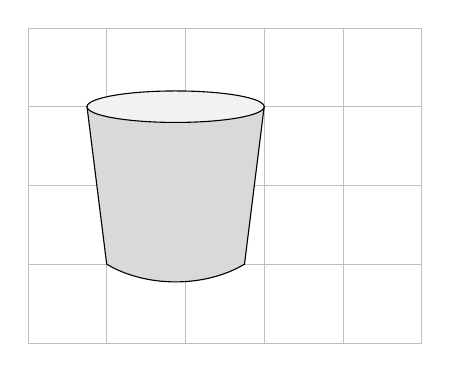
\begin{tikzpicture}

\draw [help lines,lightgray] (0,0) grid (5,4) ;
\draw[fill=gray!30] (1,1) .. controls (1.5,.7) and (2.25,.7) .. (2.75,1) -- (3,3) --  (.75,3) -- (1,1);
\draw[fill=gray!10] (1.875,3) ellipse (1.125cm and .2cm) ;

\end{tikzpicture}
}

}

\newsavebox{\fof}
\savebox{\fof}{


\scalebox{3}{

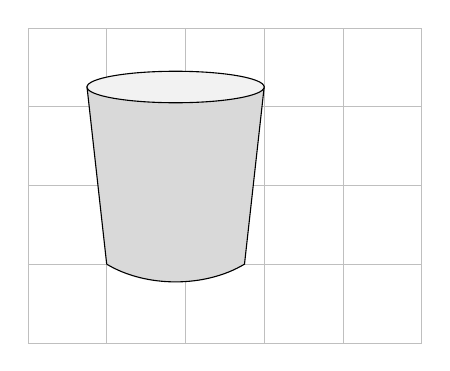
\begin{tikzpicture}

\draw [help lines,lightgray] (0,0) grid (5,4) ;
\draw[fill=gray!30] (1,1) .. controls (1.5,.7) and (2.25,.7) .. (2.75,1) -- (3,3.25) --  (.75,3.25) -- (1,1);
\draw[fill=gray!10] (1.875,3.25) ellipse (1.125cm and .2cm) ;

\end{tikzpicture}
}

}

\newsavebox{\fog}
\savebox{\fog}{


\scalebox{3}{

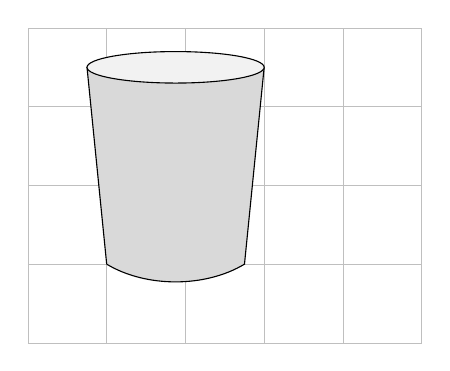
\begin{tikzpicture}

\draw [help lines,lightgray] (0,0) grid (5,4) ;
\draw[fill=gray!30] (1,1) .. controls (1.5,.7) and (2.25,.7) .. (2.75,1) -- (3,3.5) --  (.75,3.5) -- (1,1);
\draw[fill=gray!10] (1.875,3.5) ellipse (1.125cm and .2cm) ;

\end{tikzpicture}
}

}


% fifth column

\newsavebox{\fifa}
\savebox{\fifa}{


\scalebox{3}{

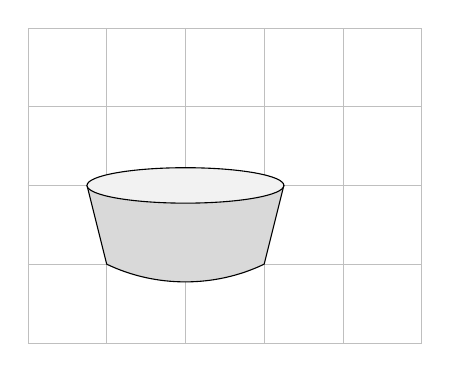
\begin{tikzpicture}

\draw [help lines,lightgray] (0,0) grid (5,4) ;
\draw[fill=gray!30] (1,1) .. controls (1.625,.7) and (2.375,.7) .. (3,1) -- (3.25,2) --  (.75,2) -- (1,1);
\draw[fill=gray!10] (2,2) ellipse (1.25cm and .225cm) ;

\end{tikzpicture}
}

}

\newsavebox{\fifb}
\savebox{\fifb}{


\scalebox{3}{

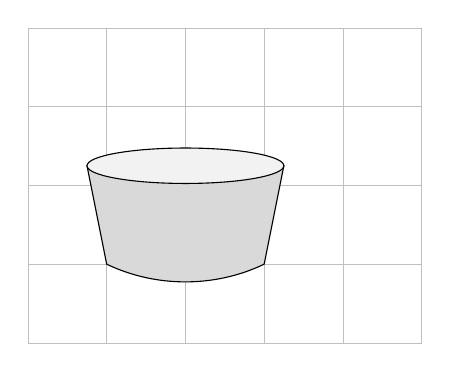
\begin{tikzpicture}

\draw [help lines,lightgray] (0,0) grid (5,4) ;
\draw[fill=gray!30] (1,1) .. controls (1.625,.7) and (2.375,.7) .. (3,1) -- (3.25,2.25) --  (.75,2.25) -- (1,1);
\draw[fill=gray!10] (2,2.25) ellipse (1.25cm and .225cm) ;

\end{tikzpicture}
}

}

\newsavebox{\fifc}
\savebox{\fifc}{


\scalebox{3}{

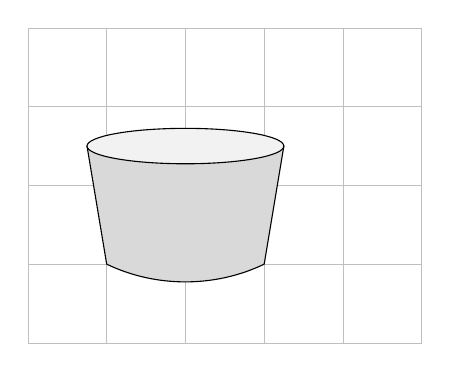
\begin{tikzpicture}

\draw [help lines,lightgray] (0,0) grid (5,4) ;
\draw[fill=gray!30] (1,1) .. controls (1.625,.7) and (2.375,.7) .. (3,1) -- (3.25,2.5) --  (.75,2.5) -- (1,1);
\draw[fill=gray!10] (2,2.5) ellipse (1.25cm and .225cm) ;

\end{tikzpicture}
}

}

\newsavebox{\fifd}
\savebox{\fifd}{


\scalebox{3}{

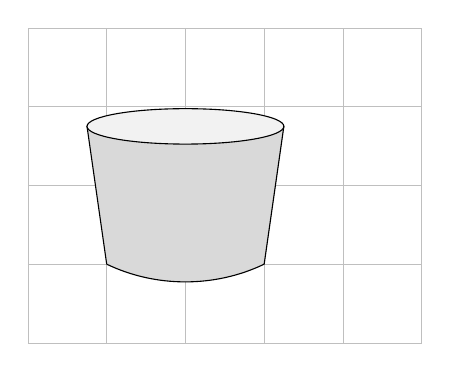
\begin{tikzpicture}

\draw [help lines,lightgray] (0,0) grid (5,4) ;
\draw[fill=gray!30] (1,1) .. controls (1.625,.7) and (2.375,.7) .. (3,1) -- (3.25,2.75) --  (.75,2.75) -- (1,1);
\draw[fill=gray!10] (2,2.75) ellipse (1.25cm and .225cm) ;

\end{tikzpicture}
}

}

\newsavebox{\fife}
\savebox{\fife}{


\scalebox{3}{

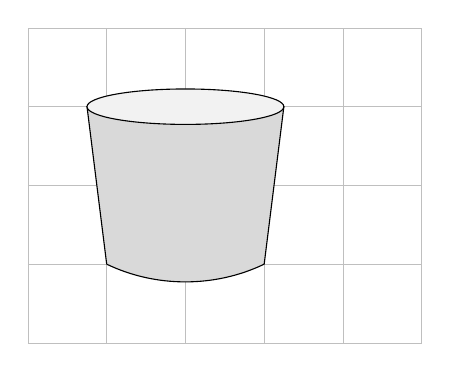
\begin{tikzpicture}

\draw [help lines,lightgray] (0,0) grid (5,4) ;
\draw[fill=gray!30] (1,1) .. controls (1.625,.7) and (2.375,.7) .. (3,1) -- (3.25,3) --  (.75,3) -- (1,1);
\draw[fill=gray!10] (2,3) ellipse (1.25cm and .225cm) ;

\end{tikzpicture}
}

}

\newsavebox{\fiff}
\savebox{\fiff}{


\scalebox{3}{

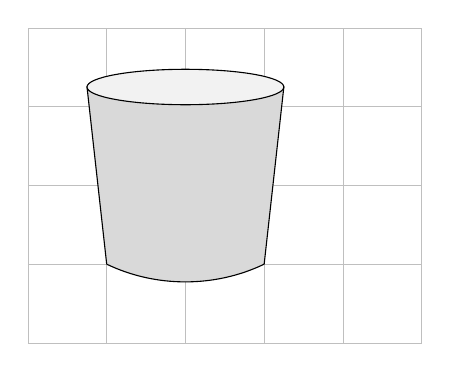
\begin{tikzpicture}

\draw [help lines,lightgray] (0,0) grid (5,4) ;
\draw[fill=gray!30] (1,1) .. controls (1.625,.7) and (2.375,.7) .. (3,1) -- (3.25,3.25) --  (.75,3.25) -- (1,1);
\draw[fill=gray!10] (2,3.25) ellipse (1.25cm and .225cm) ;

\end{tikzpicture}
}

}

\newsavebox{\fifg}
\savebox{\fifg}{


\scalebox{3}{

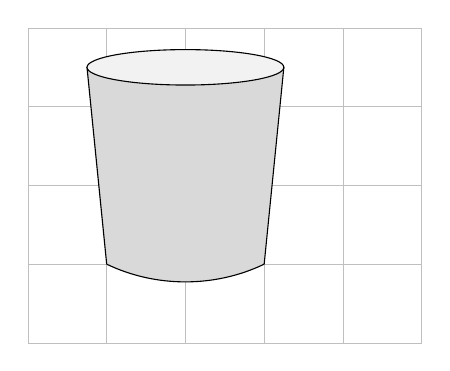
\begin{tikzpicture}

\draw [help lines,lightgray] (0,0) grid (5,4) ;
\draw[fill=gray!30] (1,1) .. controls (1.625,.7) and (2.375,.7) .. (3,1) -- (3.25,3.5) --  (.75,3.5) -- (1,1);
\draw[fill=gray!10] (2,3.5) ellipse (1.25cm and .225cm) ;

\end{tikzpicture}
}

}


%sixth column

\newsavebox{\sixa}
\savebox{\sixa}{


\scalebox{3}{

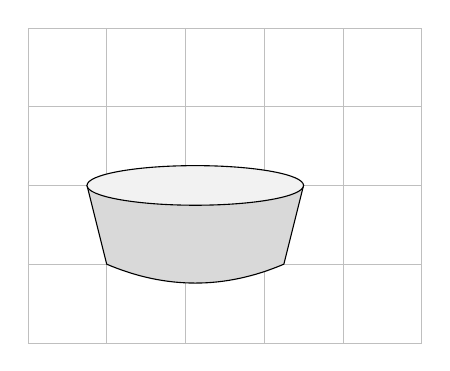
\begin{tikzpicture}

\draw [help lines,lightgray] (0,0) grid (5,4) ;
\draw[fill=gray!30] (1,1) .. controls (1.75,.68) and (2.5,.68) .. (3.25,1) -- (3.5,2) --  (.75,2) -- (1,1);
\draw[fill=gray!10] (2.125,2) ellipse (1.375cm and .2515cm) ;

\end{tikzpicture}
}

}

\newsavebox{\sixb}
\savebox{\sixb}{


\scalebox{3}{

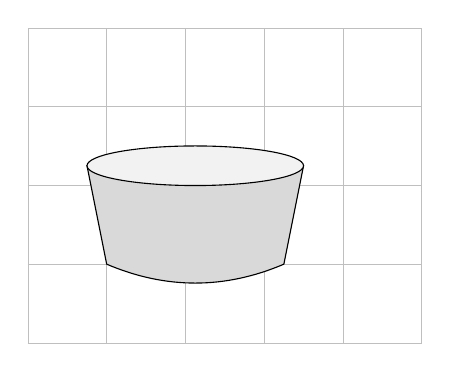
\begin{tikzpicture}

\draw [help lines,lightgray] (0,0) grid (5,4) ;
\draw[fill=gray!30] (1,1) .. controls (1.75,.68) and (2.5,.68) .. (3.25,1) -- (3.5,2.25) --  (.75,2.25) -- (1,1);
\draw[fill=gray!10] (2.125,2.25) ellipse (1.375cm and .2515cm) ;

\end{tikzpicture}
}

}

\newsavebox{\sixc}
\savebox{\sixc}{


\scalebox{3}{

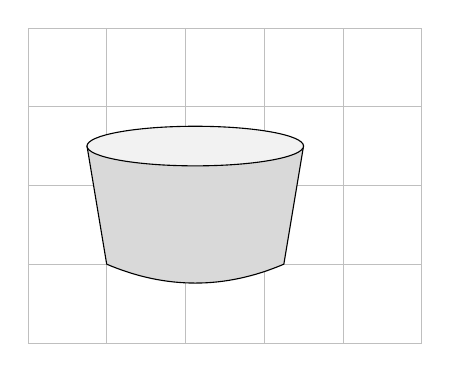
\begin{tikzpicture}

\draw [help lines,lightgray] (0,0) grid (5,4) ;
\draw[fill=gray!30] (1,1) .. controls (1.75,.68) and (2.5,.68) .. (3.25,1) -- (3.5,2.5) --  (.75,2.5) -- (1,1);
\draw[fill=gray!10] (2.125,2.5) ellipse (1.375cm and .2515cm) ;

\end{tikzpicture}
}

}

\newsavebox{\sixd}
\savebox{\sixd}{


\scalebox{3}{

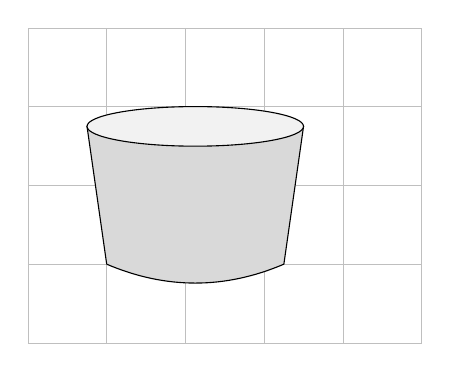
\begin{tikzpicture}

\draw [help lines,lightgray] (0,0) grid (5,4) ;
\draw[fill=gray!30] (1,1) .. controls (1.75,.68) and (2.5,.68) .. (3.25,1) -- (3.5,2.75) --  (.75,2.75) -- (1,1);
\draw[fill=gray!10] (2.125,2.75) ellipse (1.375cm and .2515cm) ;

\end{tikzpicture}
}

}

\newsavebox{\sixe}
\savebox{\sixe}{


\scalebox{3}{

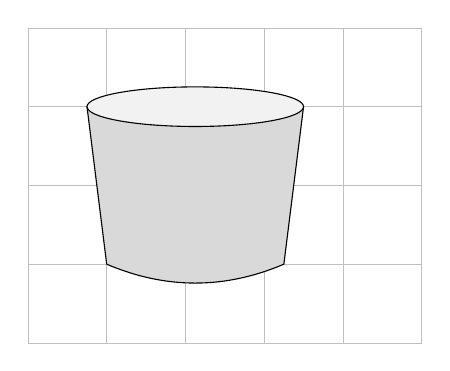
\begin{tikzpicture}

\draw [help lines,lightgray] (0,0) grid (5,4) ;
\draw[fill=gray!30] (1,1) .. controls (1.75,.68) and (2.5,.68) .. (3.25,1) -- (3.5,3) --  (.75,3) -- (1,1);
\draw[fill=gray!10] (2.125,3) ellipse (1.375cm and .2515cm) ;

\end{tikzpicture}
}

}

\newsavebox{\sixf}
\savebox{\sixf}{


\scalebox{3}{

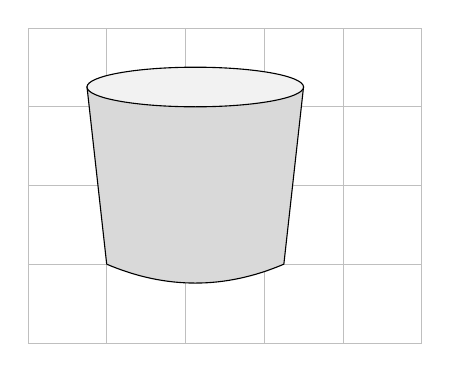
\begin{tikzpicture}

\draw [help lines,lightgray] (0,0) grid (5,4) ;
\draw[fill=gray!30] (1,1) .. controls (1.75,.68) and (2.5,.68) .. (3.25,1) -- (3.5,3.25) --  (.75,3.25) -- (1,1);
\draw[fill=gray!10] (2.125,3.25) ellipse (1.375cm and .2515cm) ;

\end{tikzpicture}
}

}

\newsavebox{\sixg}
\savebox{\sixg}{


\scalebox{3}{

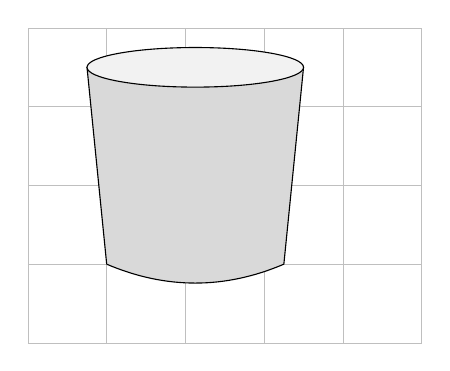
\begin{tikzpicture}

\draw [help lines,lightgray] (0,0) grid (5,4) ;
\draw[fill=gray!30] (1,1) .. controls (1.75,.68) and (2.5,.68) .. (3.25,1) -- (3.5,3.5) --  (.75,3.5) -- (1,1);
\draw[fill=gray!10] (2.125,3.5) ellipse (1.375cm and .2515cm) ;

\end{tikzpicture}
}

}



% seventh column

\newsavebox{\seva}
\savebox{\seva}{


\scalebox{3}{

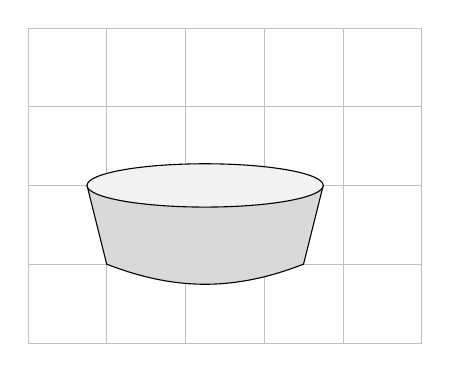
\begin{tikzpicture}

\draw [help lines,lightgray] (0,0) grid (5,4) ;
\draw[fill=gray!30] (1,1) .. controls (1.875,.66) and (2.625,.66) .. (3.5,1) -- (3.75,2) --  (.75,2) -- (1,1);
\draw[fill=gray!10] (2.25,2) ellipse (1.5cm and .275cm) ;

\end{tikzpicture}
}

}

\newsavebox{\sevb}
\savebox{\sevb}{


\scalebox{3}{

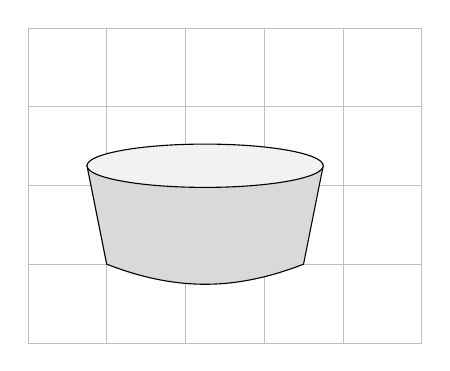
\begin{tikzpicture}

\draw [help lines,lightgray] (0,0) grid (5,4) ;
\draw[fill=gray!30] (1,1) .. controls (1.875,.66) and (2.625,.66) .. (3.5,1) -- (3.75,2.25) --  (.75,2.25) -- (1,1);
\draw[fill=gray!10] (2.25,2.25) ellipse (1.5cm and .275cm) ;

\end{tikzpicture}
}

}

\newsavebox{\sevc}
\savebox{\sevc}{


\scalebox{3}{

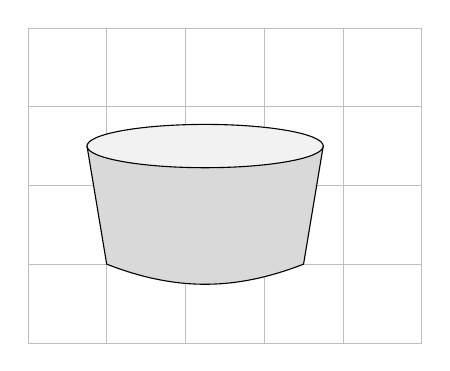
\begin{tikzpicture}

\draw [help lines,lightgray] (0,0) grid (5,4) ;
\draw[fill=gray!30] (1,1) .. controls (1.875,.66) and (2.625,.66) .. (3.5,1) -- (3.75,2.5) --  (.75,2.5) -- (1,1);
\draw[fill=gray!10] (2.25,2.5) ellipse (1.5cm and .275cm) ;

\end{tikzpicture}
}

}

\newsavebox{\sevd}
\savebox{\sevd}{


\scalebox{3}{

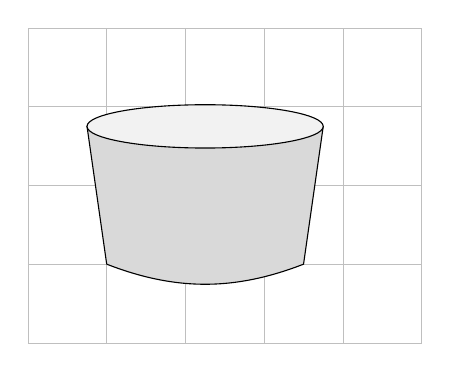
\begin{tikzpicture}

\draw [help lines,lightgray] (0,0) grid (5,4) ;
\draw[fill=gray!30] (1,1) .. controls (1.875,.66) and (2.625,.66) .. (3.5,1) -- (3.75,2.75) --  (.75,2.75) -- (1,1);
\draw[fill=gray!10] (2.25,2.75) ellipse (1.5cm and .275cm) ;

\end{tikzpicture}
}

}

\newsavebox{\seve}
\savebox{\seve}{


\scalebox{3}{

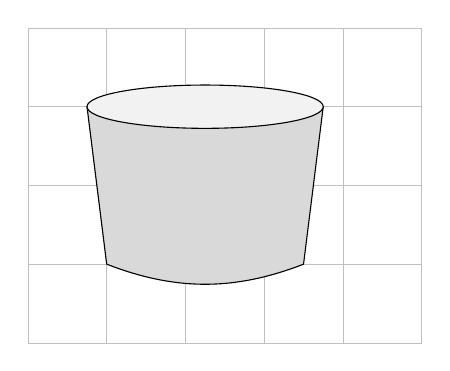
\begin{tikzpicture}

\draw [help lines,lightgray] (0,0) grid (5,4) ;
\draw[fill=gray!30] (1,1) .. controls (1.875,.66) and (2.625,.66) .. (3.5,1) -- (3.75,3) --  (.75,3) -- (1,1);
\draw[fill=gray!10] (2.25,3) ellipse (1.5cm and .275cm) ;

\end{tikzpicture}
}

}

\newsavebox{\sevf}
\savebox{\sevf}{


\scalebox{3}{

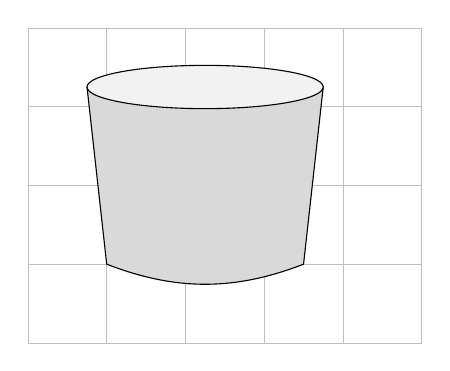
\begin{tikzpicture}

\draw [help lines,lightgray] (0,0) grid (5,4) ;
\draw[fill=gray!30] (1,1) .. controls (1.875,.66) and (2.625,.66) .. (3.5,1) -- (3.75,3.25) --  (.75,3.25) -- (1,1);
\draw[fill=gray!10] (2.25,3.25) ellipse (1.5cm and .275cm) ;

\end{tikzpicture}
}

}

\newsavebox{\sevg}
\savebox{\sevg}{


\scalebox{3}{

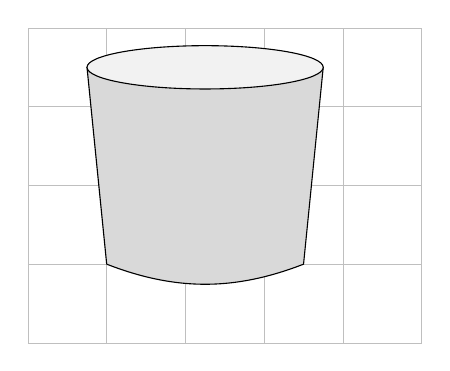
\begin{tikzpicture}

\draw [help lines,lightgray] (0,0) grid (5,4) ;
\draw[fill=gray!30] (1,1) .. controls (1.875,.66) and (2.625,.66) .. (3.5,1) -- (3.75,3.5) --  (.75,3.5) -- (1,1);
\draw[fill=gray!10] (2.25,3.5) ellipse (1.5cm and .275cm) ;

\end{tikzpicture}
}

}

\newsavebox{\nsone}
\savebox{\nsone}{


\scalebox{3}{

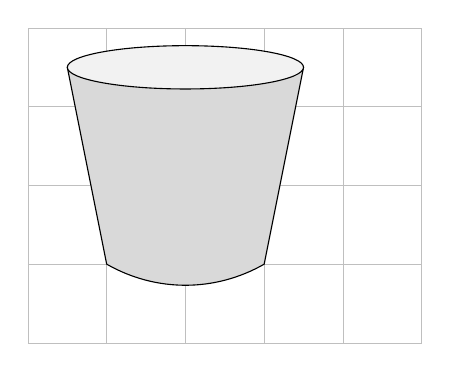
\begin{tikzpicture}

\draw [help lines,lightgray] (0,0) grid (5,4) ;
\draw[fill=gray!30] (1,1) .. controls (1.625,.643) and (2.375,.643) .. (3,1) -- (3.5,3.5) --  (.5,3.5) -- (1,1);
\draw[fill=gray!10] (2,3.5) ellipse (1.5cm and .275cm) ;

\end{tikzpicture}
}

}

\newsavebox{\nstwo}
\savebox{\nstwo}{


\scalebox{3}{

\begin{tikzpicture}

\draw [help lines,lightgray] (0,0) grid (5,4) ;
\draw[fill=gray!30] (1,1) .. controls (1.125,.75) and (1.875,.75) .. (2,1) -- (2.1,2.25) --  (.9,2.25) -- (1,1);
\draw[fill=gray!10] (1.5,2.25) ellipse (.6cm and .125cm) ;

\end{tikzpicture}
}

}

\newsavebox{\nsthree}
\savebox{\nsthree}{


\scalebox{3}{

\begin{tikzpicture}

\draw [help lines,lightgray] (0,0) grid (5,4) ;
\draw[fill=gray!30] (1,1) .. controls (1.125,.75) and (1.875,.75) .. (2,1) -- (2.1,3.25) --  (.9,3.25) -- (1,1);
\draw[fill=gray!10] (1.5,3.25) ellipse (.6cm and .135cm) ;

\end{tikzpicture}
}

}

\newsavebox{\nsfour}
\savebox{\nsfour}{


\scalebox{3}{

\begin{tikzpicture}

\draw [help lines,lightgray] (0,0) grid (5,4) ;
\draw[fill=gray!30] (1,1) .. controls (1.8,.785) and (2.45,.785) .. (3.25,1) -- (3.3,1.7) --  (.95,1.7) -- (1,1);
\draw[fill=gray!10] (2.125,1.7) ellipse (1.175cm and .185cm) ;

\end{tikzpicture}
}

}

\newsavebox{\nsfive}
\savebox{\nsfive}{


\scalebox{3}{

\begin{tikzpicture}

\draw [help lines,lightgray] (0,0) grid (5,4) ;
\draw[fill=gray!30] (1,1) .. controls (1.5,.7725) and (2.25,.7725) .. (2.75,1) -- (2.75,1.9) --  (1,1.9) -- (1,1);
\draw[fill=gray!10] (1.875,1.9) ellipse (.875cm and .175cm) ;

\end{tikzpicture}
}

}

\newsavebox{\nssix}
\savebox{\nssix}{


\scalebox{3}{

\begin{tikzpicture}

\draw [help lines,lightgray] (0,0) grid (5,4) ;
\draw[fill=gray!30] (1.15,1) .. controls (1.23,.76) and (1.77,.76) .. (1.85,1) -- (2.25,3.65) --  (.75,3.65) -- (1.15,1);
\draw[fill=gray!10] (1.5,3.65) ellipse (.75cm and .15cm) ;

\end{tikzpicture}
}

}

\newsavebox{\nsseven}
\savebox{\nsseven}{


\scalebox{3}{

\begin{tikzpicture}

\draw [help lines,lightgray] (0,0) grid (5,4) ;
\draw[fill=gray!30] (1.15,1) .. controls (1.4,.875) and (1.6,.875) .. (1.85,1) -- (2.75,3) --  (.25,3) -- (1.15,1);
\draw[fill=gray!10] (1.5,3) ellipse (1.25cm and .185cm) ;

\end{tikzpicture}
}

}

\newsavebox{\nseight}
\savebox{\nseight}{


\scalebox{3}{

\begin{tikzpicture}

\draw [help lines,lightgray] (0,0) grid (5,4) ;
\draw[fill=gray!30] (1,1) .. controls (1.62,.797) and (2.38,.797) .. (3,1) -- (3.25,1.43) --  (.75,1.43) -- (1,1);
\draw[fill=gray!10] (2,1.43) ellipse (1.25cm and .175cm) ;

\end{tikzpicture}
}

}

\newsavebox{\nsnine}
\savebox{\nsnine}{


\scalebox{3}{

\begin{tikzpicture}

\draw [help lines,lightgray] (0,0) grid (5,4) ;
\draw[fill=gray!30] (1,1) .. controls (1.5,.69) and (3.5,.69) .. (4,1) -- (4,2) --  (1,2) -- (1,1);
\draw[fill=gray!10] (2.5,2) ellipse (1.5cm and .255cm) ;

\end{tikzpicture}
}

}

\newsavebox{\nsten}
\savebox{\nsten}{


\scalebox{3}{

\begin{tikzpicture}

\draw [help lines,lightgray] (0,0) grid (5,4) ;
\draw[fill=gray!30] (1.15,1) .. controls (1.23,.76) and (1.77,.76) .. (1.85,1) -- (2.5,2.45) --  (.5,2.45) -- (1.15,1);
\draw[fill=gray!10] (1.5,2.45) ellipse (1cm and .135cm) ;

\end{tikzpicture}
}

}

\newsavebox{\nseleven}
\savebox{\nseleven}{


\scalebox{3}{

\begin{tikzpicture}

\draw [help lines,lightgray] (0,0) grid (5,4) ;
\draw[fill=gray!30] (1.15,1) .. controls (1.26,.87) and (1.74,.87) .. (1.85,1) -- (2.5,1.5) --  (.5,1.5) -- (1.15,1);
\draw[fill=gray!10] (1.5,1.5) ellipse (1cm and .135cm) ;

\end{tikzpicture}
}

}

\newsavebox{\nstwelve}
\savebox{\nstwelve}{


\scalebox{3}{

\begin{tikzpicture}

\draw [help lines,lightgray] (0,0) grid (5,4) ;
\draw[fill=gray!30] (1.15,1) .. controls (1.25,.82) and (1.75,.82) .. (1.85,1) -- (2.25,2.6) --  (.75,2.6) -- (1.15,1);
\draw[fill=gray!10] (1.5,2.6) ellipse (.75cm and .15cm) ;

\end{tikzpicture}
}

}

\newsavebox{\nsthirteen}
\savebox{\nsthirteen}{


\scalebox{3}{

\begin{tikzpicture}

\draw [help lines,lightgray] (0,0) grid (5,4) ;
\draw[fill=gray!30] (1,1) .. controls (1.375,.7) and (2.125,.7)  .. (2.5,1) -- (2.5,1.5) --  (1,1.5) -- (1,1);
\draw[fill=gray!10] (1.75,1.5) ellipse (.75cm and .195cm) ;

\end{tikzpicture}
}

}

\newsavebox{\nsfourteen}
\savebox{\nsfourteen}{


\scalebox{3}{

\begin{tikzpicture}

\draw [help lines,lightgray] (0,0) grid (5,4) ;
\draw[fill=gray!30] (1.1,1) .. controls (1.3,.8) and (1.95,.8) .. (2.15,1) -- (2.35,3.1) --  (.9,3.1) -- (1.1,1);
\draw[fill=gray!10] (1.625,3.1) ellipse (.73cm and .175cm) ;

\end{tikzpicture}
}

}

\newsavebox{\nsfifteen}
\savebox{\nsfifteen}{


\scalebox{3}{

\begin{tikzpicture}

\draw [help lines,lightgray] (0,0) grid (5,4) ;
\draw[fill=gray!30] (1,1) .. controls (1.5,.7) and (2.75,.7) .. (3.25,1) -- (4.25,2.7) --  (0,2.7) -- (1,1);
\draw[fill=gray!10] (2.125,2.7) ellipse (2.125cm and .2cm) ;

\end{tikzpicture}
}

}


\newsavebox{\nssixteen}
\savebox{\nssixteen}{


\scalebox{3}{

\begin{tikzpicture}

\draw [help lines,lightgray] (0,0) grid (5,4) ;
\draw[fill=gray!30] (1,1) .. controls (1.875,.68) and (2.625,.68) .. (3.5,1) -- (3.6,2.15) --  (.9,2.15) -- (1,1);
\draw[fill=gray!10] (2.25,2.15) ellipse (1.35cm and .275cm) ;

\end{tikzpicture}
}

}


%%%%%%%%%%%%%%%%%%%%%%%%%%%%%%%%%%%%%%%%%



\begin{picture}(250,250)
	\put(-50,-150){\usebox{\nsone}}
\end{picture}


\newpage


\begin{picture}(250,250)
	\put(-50,-150){\usebox{\nstwo}}
\end{picture}


\newpage


\begin{picture}(250,250)
	\put(-50,-150){\usebox{\nsthree}}
\end{picture}


\newpage


\begin{picture}(250,250)
	\put(-50,-150){\usebox{\nsfour}}
\end{picture}




\newpage


\begin{picture}(250,250)
	\put(-50,-150){\usebox{\nsfive}}
\end{picture}



\newpage


\begin{picture}(250,250)
	\put(-50,-150){\usebox{\nssix}}
\end{picture}


\newpage


\begin{picture}(250,250)
	\put(-50,-150){\usebox{\nsseven}}
\end{picture}


\newpage


\begin{picture}(250,250)
	\put(-50,-150){\usebox{\nseight}}
\end{picture}


\newpage


\begin{picture}(250,250)
	\put(-50,-150){\usebox{\nsnine}}
\end{picture}


\newpage


\begin{picture}(250,250)
	\put(-50,-150){\usebox{\nsten}}
\end{picture}


\newpage


\begin{picture}(250,250)
	\put(-50,-150){\usebox{\nseleven}}
\end{picture}


\newpage


\begin{picture}(250,250)
	\put(-50,-150){\usebox{\nstwelve}}
\end{picture}


\newpage


\begin{picture}(250,250)
	\put(-50,-150){\usebox{\nsthirteen}}
\end{picture}


\newpage


\begin{picture}(250,250)
	\put(-50,-150){\usebox{\nsfourteen}}
\end{picture}


\newpage


\begin{picture}(250,250)
	\put(-50,-150){\usebox{\nsfifteen}}
\end{picture}


\newpage


\begin{picture}(250,250)
	\put(-50,-150){\usebox{\nssixteen}}
\end{picture}


\end{document}
